\chapter{Possible implementations}
This chapter will discuss the potential implementations of the partial mesh star topology within the context of a computer network dedicated to energy monitoring. The network primarily consists of the Area Control Center, primary stations, and secondary stations, each managed by its own Kubernetes cluster.

\section{Logical domains}
The Area Control Center occupies the central position in the star topology, establishing unidirectional peering with offloading to every other entity in the topology, whether it is a primary station or a secondary station. This allows the Area Control Center to manage all application deployments without the need to delegate them to other nodes.

The remaining clusters are divided into groups, typically consisting of a primary station and its associated secondary stations. These groups represent a logical domain of applications with their own high-availability distributed database system and, therefore, do not have interconnections among them. Within a group, the clusters form a full mesh of unidirectional peerings for the database system's operation, and they share the same offloaded namespace from the Area Control Center. 

This implementation is depicted in Figure~\ref{fig:domains}.

\begin{figure}[ht]\centering
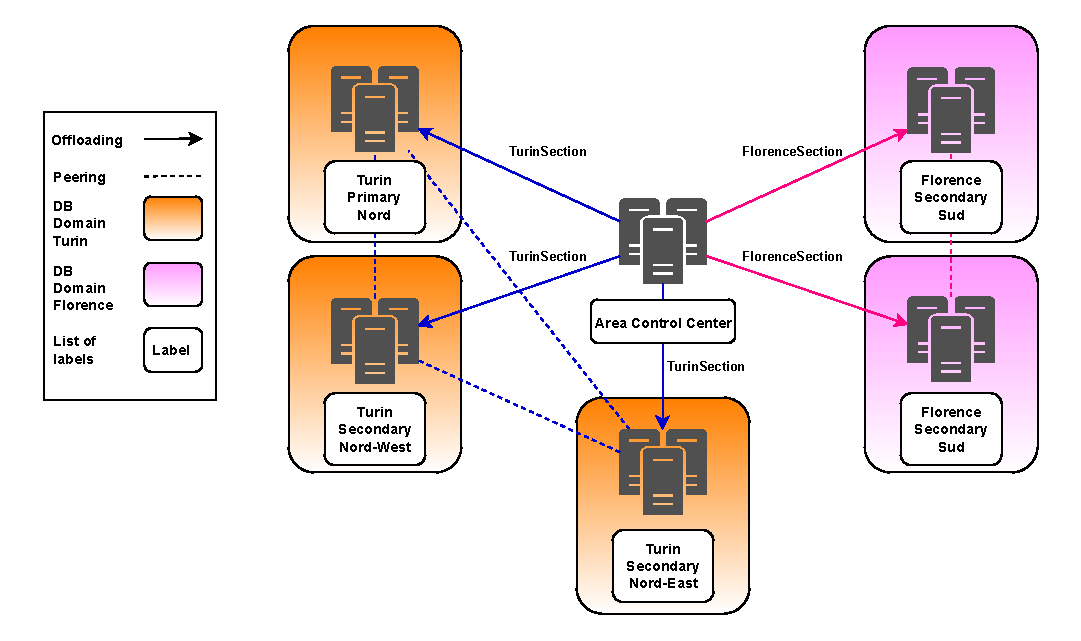
\includegraphics[scale=0.7]{Pictures/Domain-v3}
\caption{Logical domains scheme}\label{fig:domains}
\end{figure}

\subsection{Logical domains analysis}

This architecture allows for the highest degree of resilience, as considering every possible failure in the control and power distribution network infrastructure, represented in Figure~\ref{fig:failures}, the only fault that is not automatically recoverable is the disconnection of the Area Control Center.

\begin{figure}[ht]\centering
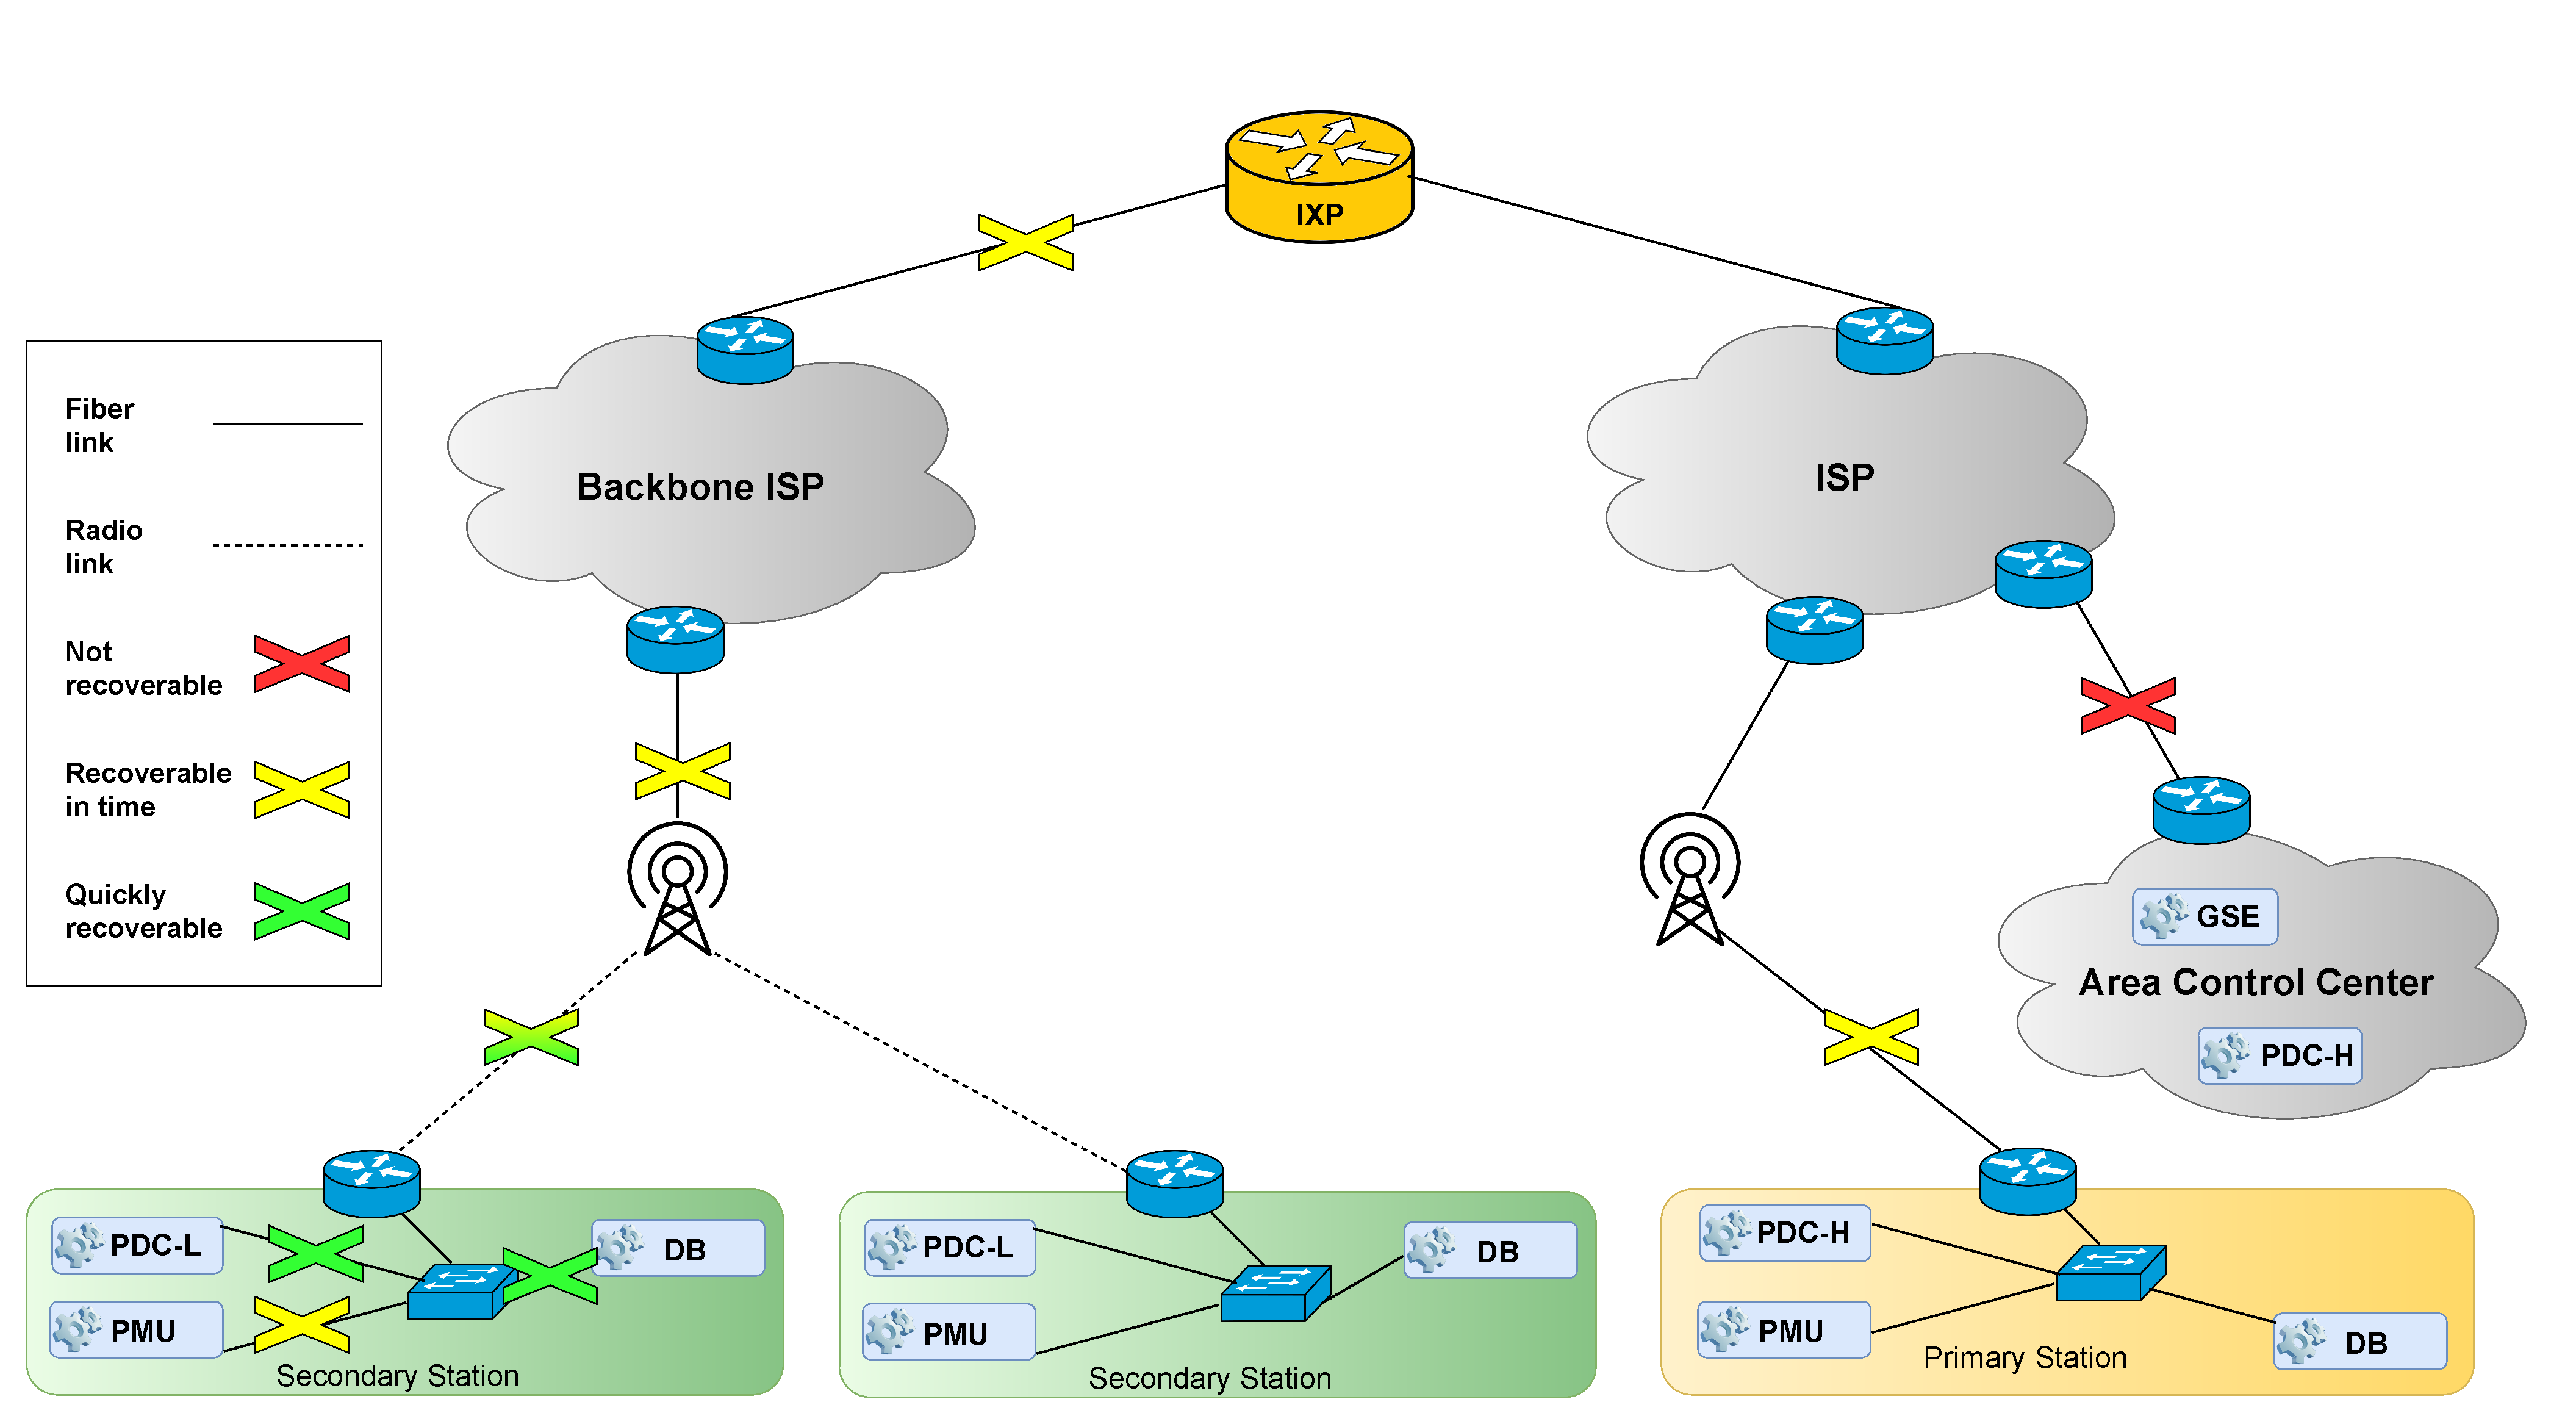
\includegraphics[scale=0.20]{Pictures/failures}
\caption{Possible failures in logical domains implementation}\label{fig:failures}
\end{figure}

The cluster representing the Area Control Center is a critical point as it hosts the central logic of the network, but the effects of a failure or disconnection of this node are negligible when compared to environmental constraints:

\begin{enumerate}
\item In the event of a physical failure of the central node, deployments would be lost, making the reconciliation process with the entire network impossible. However, this is negligible because without the central node's logic, the network would not be observable by default.
\item In the event of a complete disconnection from the network, active workloads would continue to function, but the reconciliation process for stateful applications (as the database system) will not occur since, by the point of view of the deployments, there would not be enough surviving replicas to maintain the system. Yet, this is also negligible as it falls under the same scenario as before.
\end{enumerate}

In contrast, all other failures are recoverable from the perspective of the Area Control Center. Failures within a cluster are generally recoverable in a short time as the applications are automatically and quickly ricreated into a healthy node (which can belong to either the local cluster or a remote cluster) in case of disconnection or internal pod failure. 

Disconnections of nodes, entire clusters, or parts of the network containing data production sources (PMUs) are automatically recoverable only with the restoration of the connection itself, as the PMU is physical hardware tied to its node and cannot be moved to others.

The aforementioned concerns the perspective of the Area Control Center, but as described in the previous chapter, the disconnected part of the network continues to function perfectly, and thanks to Liqo technology, additional applications can be instantiated to support the temporary independence of the network.

The continuation of operations can be observed in Figure~\ref{fig:stream}, which illustrates the data stream about frequency values seen by an instance of PDC lower and its directly superior PDC higher, shortly before and shortly after the disconnection of the cluster hosting the PDC lower and its data sources, which occurred at 44,633 s. PDC lower continues to receive data from the sources, operating in an isolated environment, while PDC higher stops receiving the data stream from the isolated source. 

\begin{figure}[ht]\centering
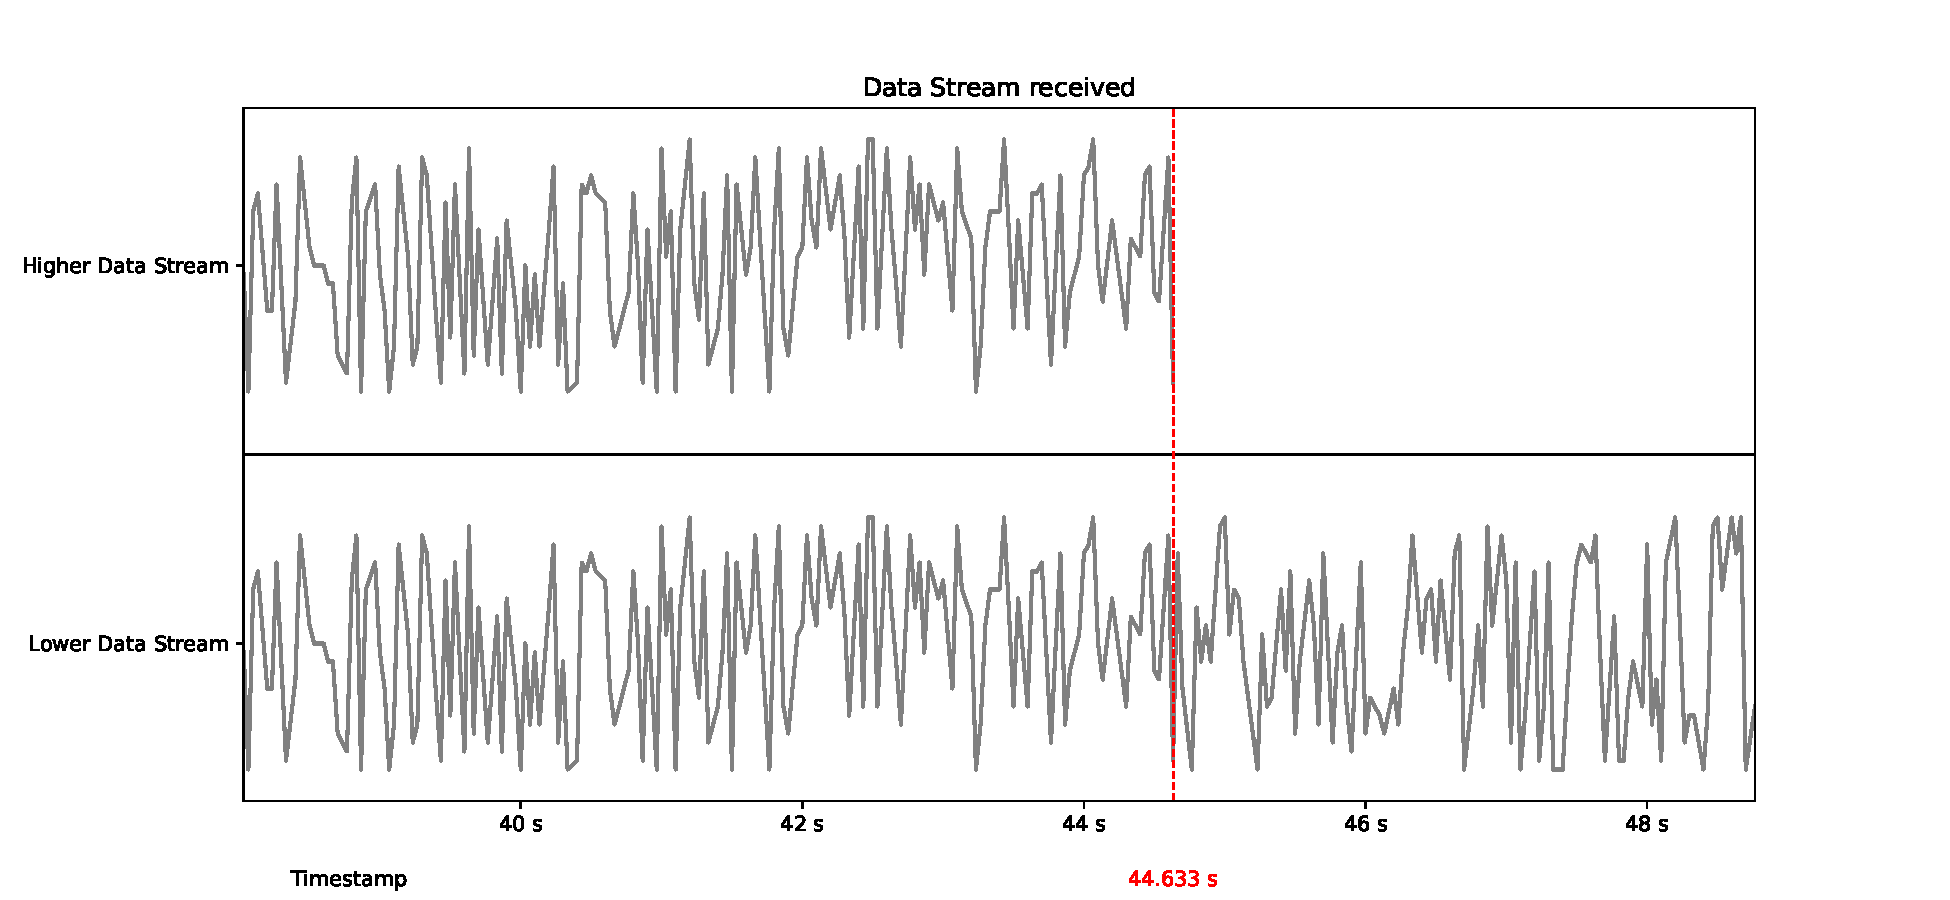
\includegraphics[scale=0.5]{Pictures/data-stream}
\caption{Data Stream comparison in case of failure}\label{fig:stream}
\end{figure}

The limitations of this architecture pertain to scalability, as each cluster requires its own distinct CIDR for the transparent operation of high-availability distributed database systems. Additionally, each peering creates a virtual representative node in the central cluster, limiting the number of possible clusters to 5000, according to the official Kubernetes documentation.

\section{Multi-level logical domains}
The implementation described in this section leverages a star topology twice, once with a partial mesh version and once with a full version, as shown in Figure~\ref{fig:level-imp}. This follows the division of stations into primary and secondary, although it could be adapted to n subdivisions.

The first topology used is a partial mesh star topology used to connect the Area Control Center (central cluster) with all primary stations (leaf clusters). The central cluster handles the deployment of high-level applications along with their respective distributed database systems, offloading the corresponding namespace through peering to the respective group of primary stations.

The groups of primary stations are composed of a main primary station, where workload is preferably directed (using labels), while the others in the group primarily serve as backups in case of failure of the main station. This means that primary stations can be in multiple groups, one where they are primary and others where they function as backups, leveraging the topology seen in Chapter~\ref{chap:partial-mesh-star} section~\ref{sec:indipendent-groups}.

\begin{figure}[ht]\centering
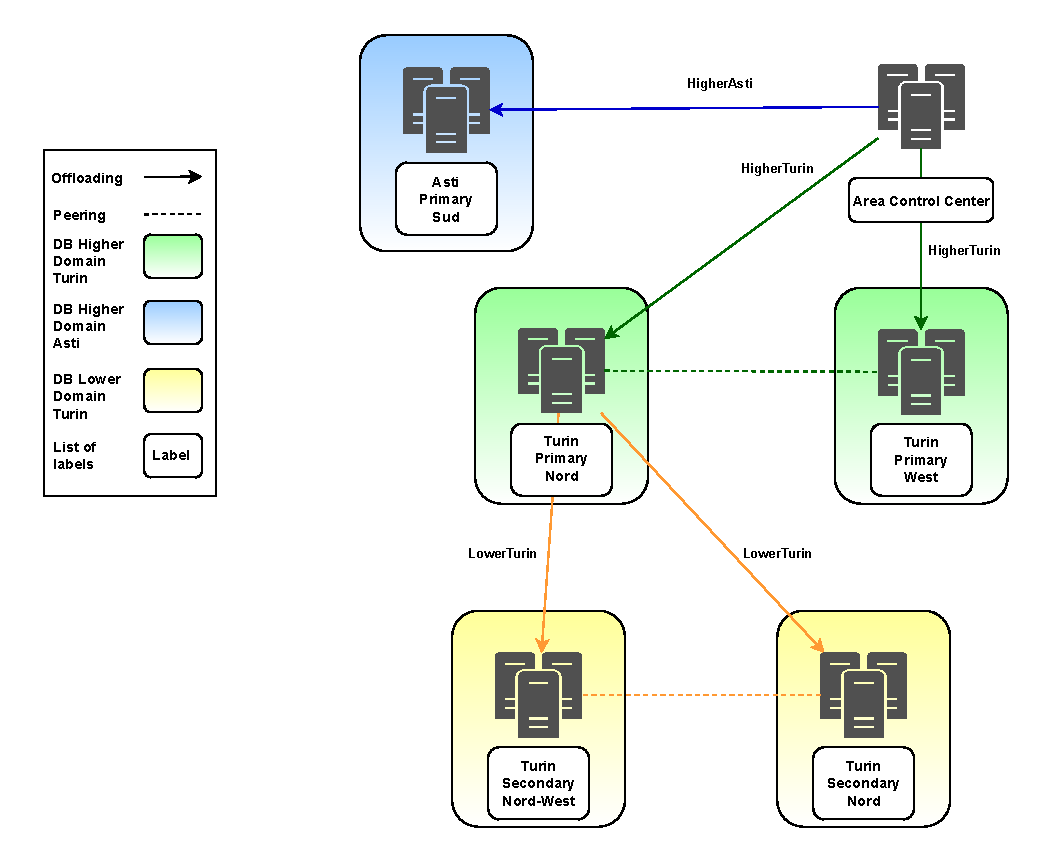
\includegraphics[scale=0.5]{Pictures/2level}
\caption{2 Level logical domains }\label{fig:level-imp}
\end{figure}

The main primary station of each group also serves as the central cluster in the second star topology, connecting not only to the backup primary stations but also to all secondary stations under its jurisdiction. In our implementation, this will be a full mesh star topology, but a partial mesh could also be used if the secondary stations do not share the same distributed database system.

In this second topology, the main primary station handles the deployment of low-level applications along with their respective high-availability distributed databases, consequently offloading the namespace to its secondary stations. The data stream for monitoring, which passes through two different namespaces (from the low-level to the high-level), relies on external exposure services such as load balancers and ingress, enabling access to the high-level application whether it resides in the primary station or, due to a failure, in one of the backup primary stations.


\subsection{Multi-level logical domains analysis}

This architecture enhances scalability limits compared to the previous implementation by reducing the number of peerings managed by the Area Control Center and requiring distinct CIDRs only within the secondary topologies associated with a primary station, allowing for reuse across different types.

However, this benefit is balanced by a decrease in overall resilience, because in addition to the critical point represented by the Area Control Center, all primary stations that manage a subnetwork of secondary stations also become critical points, as shown in Figure~\ref{fig:failures2}.

This is because a failure or disconnection of the primary station results in the loss of deployment for low-level applications, which is not a feature supported by Liqo technology, thus necessitating a system reset upon reconnection.

\begin{figure}[ht]\centering
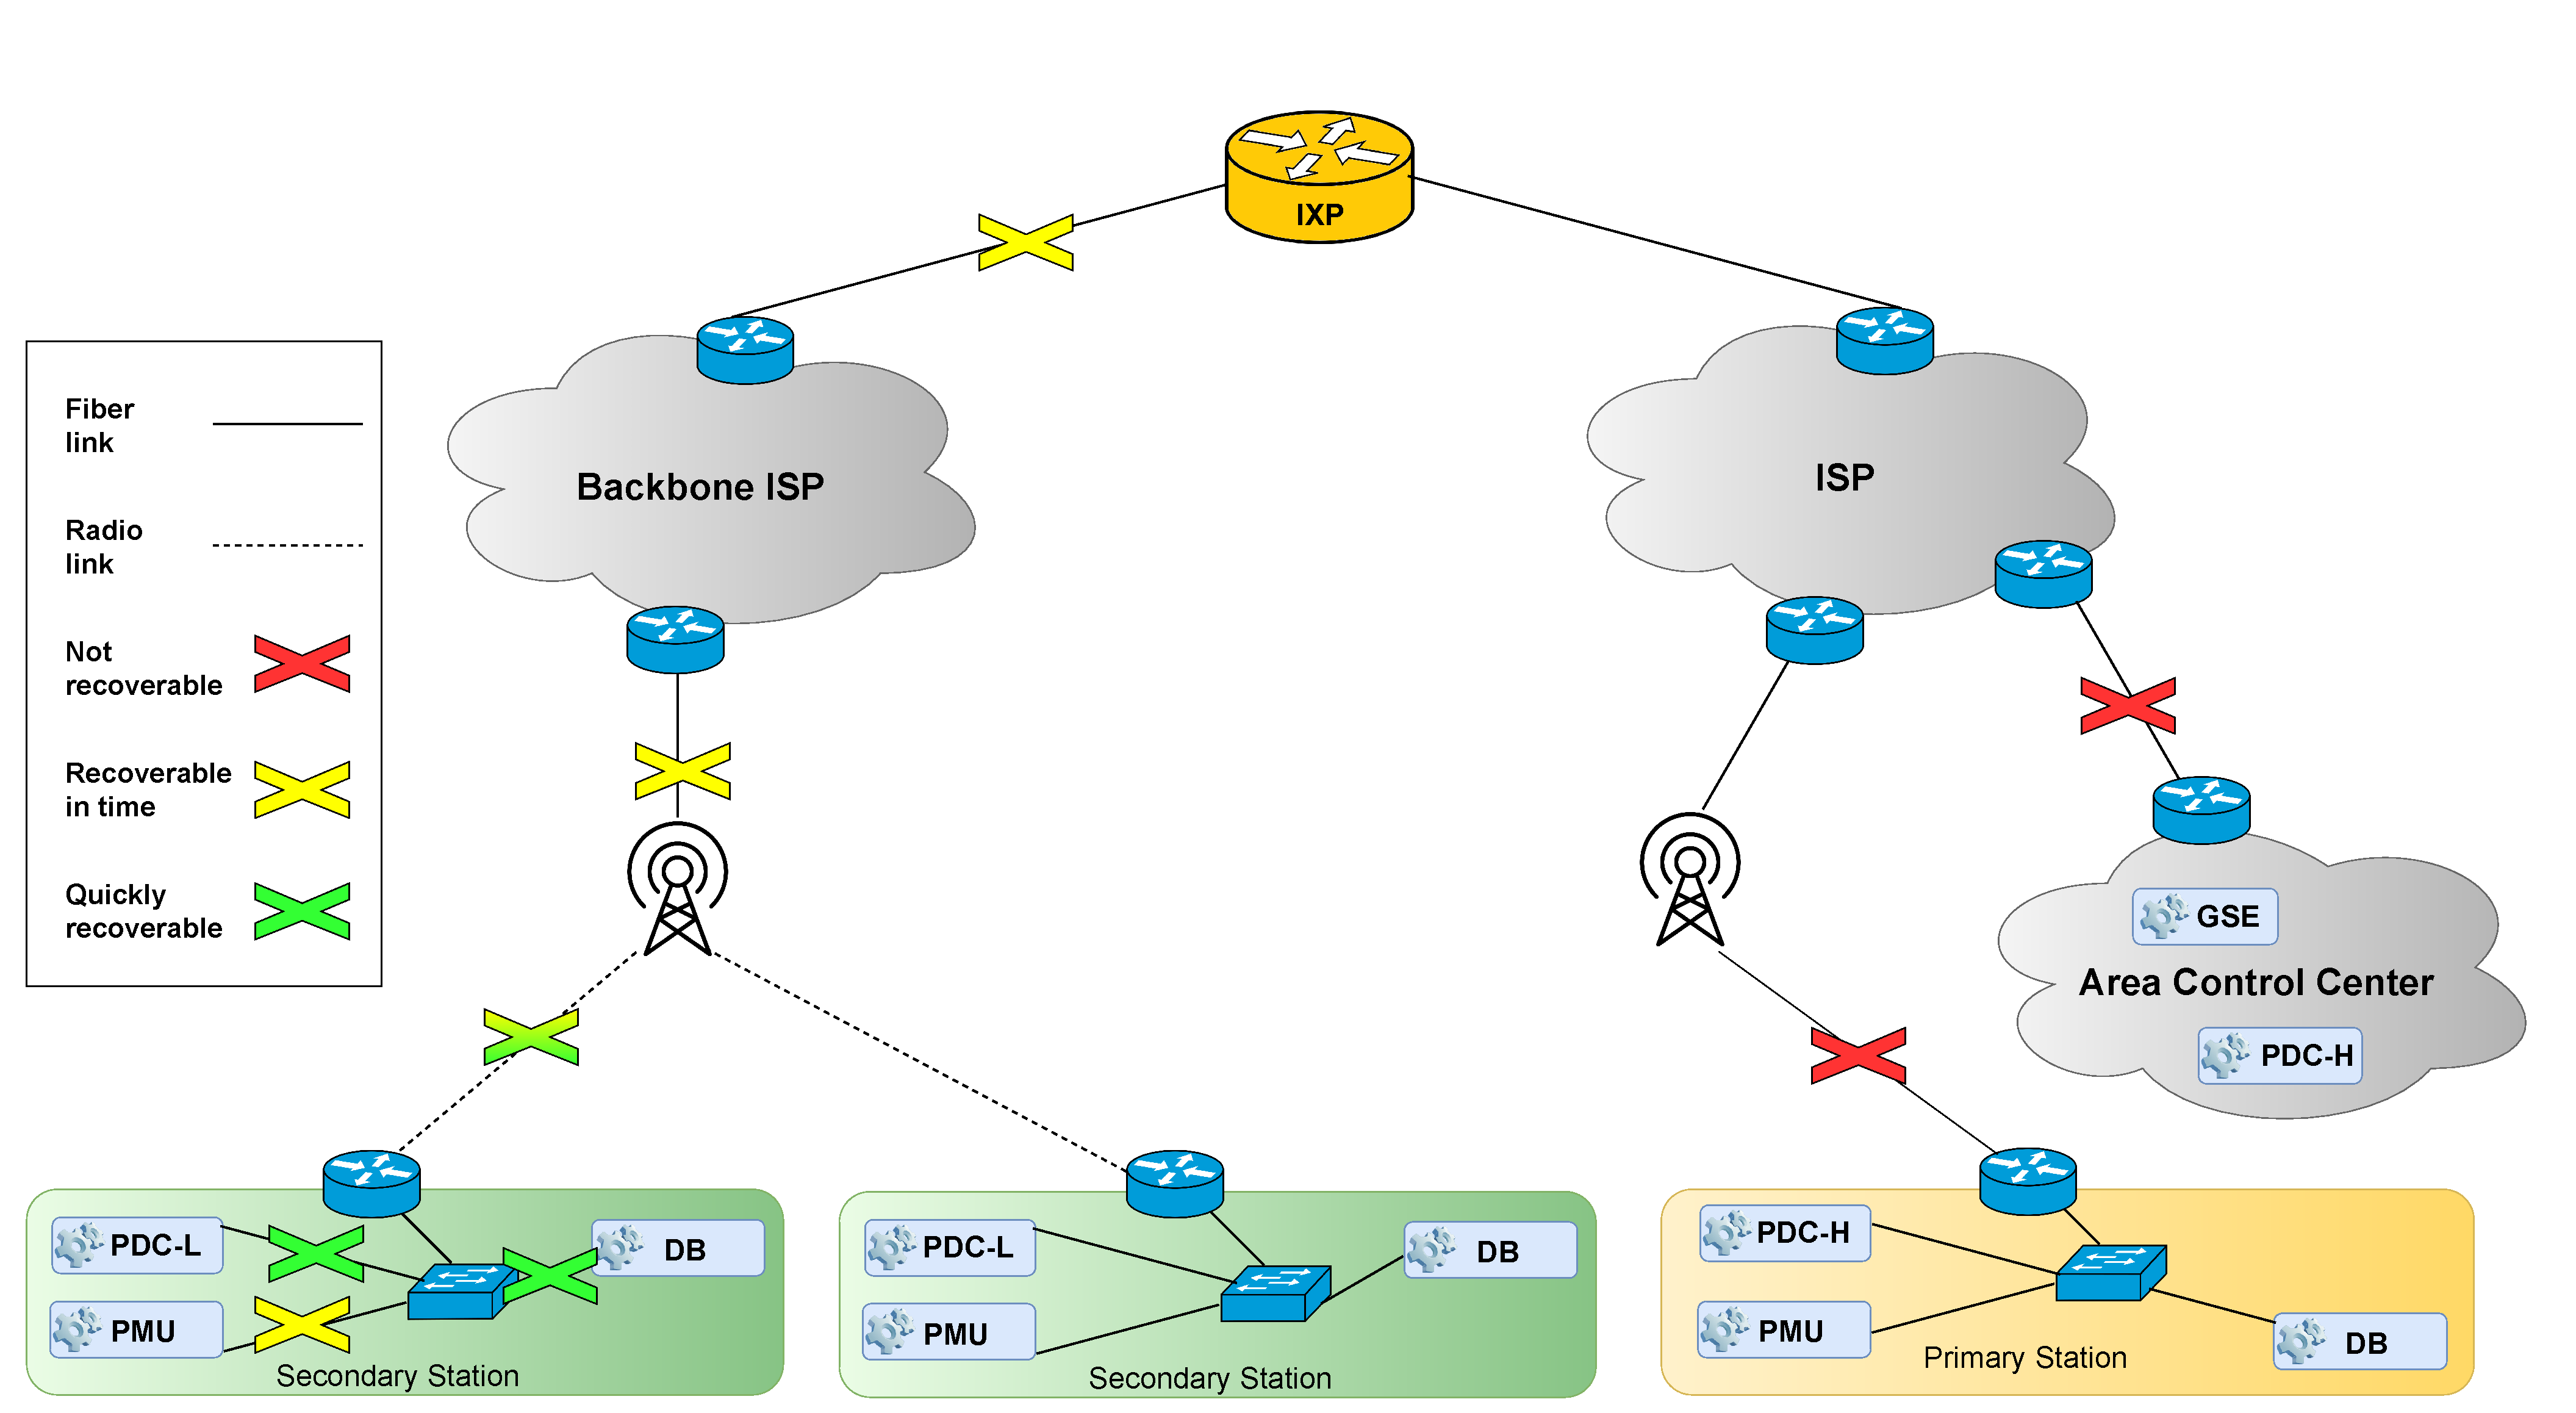
\includegraphics[scale=0.20]{Pictures/failures2}
\caption{Possible failures in multi-level logical domains implementation}\label{fig:failures2}
\end{figure}

This thesis focuses on achieving the highest degree of resilience; therefore, the following chapter will focus on testing the first implementation. It is important to note that these two implementations are not mutually exclusive; they can be implemented simultaneously within the same physical network, in cases where different parts of the network require varying degrees of resilience.